\subsection{Configurazione ambiente di sviluppo integrato WebStorm}
La configurazione minima di WebStorm prevede la corretta configurazione dei path di sistema e l'apertura di un progetto.
\subsubsection{Configurazione dei path di sistema}
Aprire le impostazioni di WebStorm dal suo menù "File" ed utilizzando la barra di ricerca cercare "Node.js and NPM". Verificare quindi che entrambe le voci "Node interpreter" e "Package manager" siano correttamente impostate.
\\
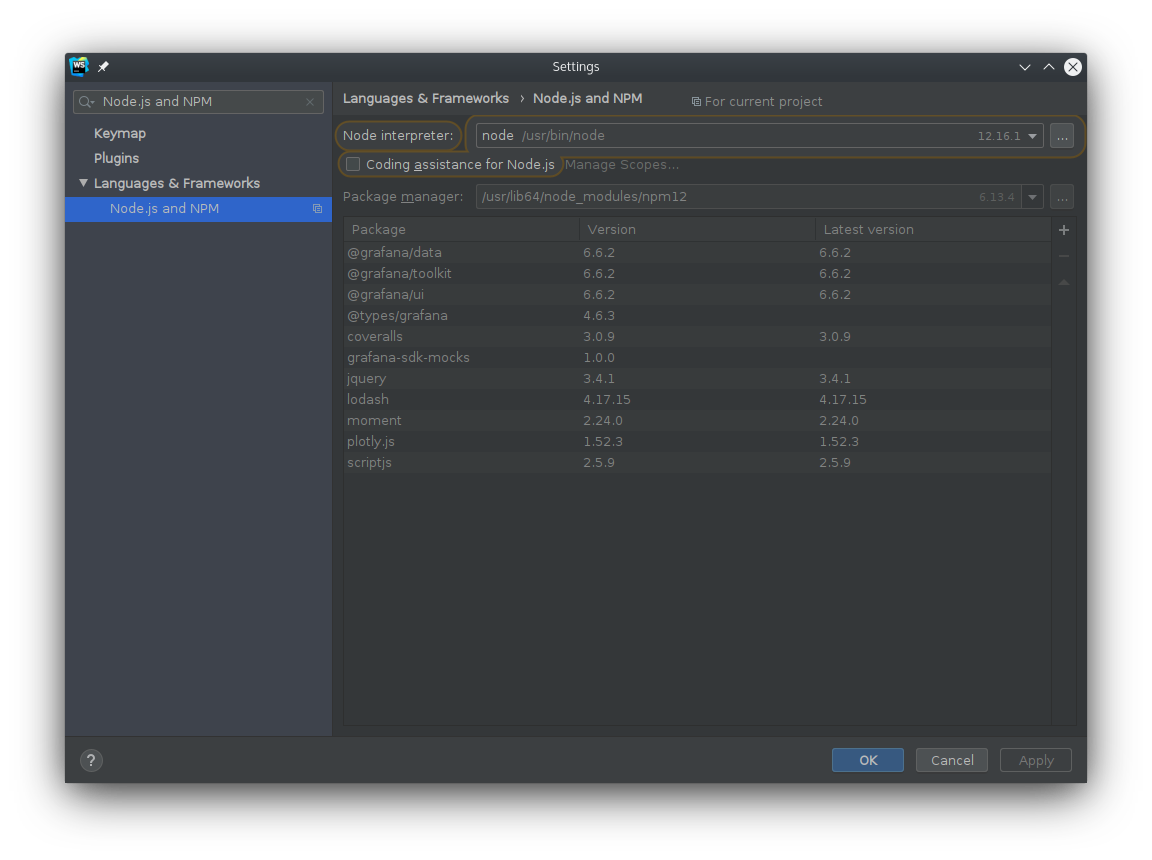
\includegraphics[width=\textwidth,height=\textheight,keepaspectratio]{img/node-npm.png}
\subsubsection{Importazione di un progetto}
Dal menu "File" selezionare la voce "Open" e selezionare quindi la root directory del repository desiderato.
\subsection{Configurazione plugin SonarLint per WebStorm}
\subsubsection{Configurazione globale}
Per configurare il plugin SonarLint per WebStorm aprire le impostazioni di WebStorm dal suo menù "File", Quindi nella sezione "Tools" selezionare la voce "SonarLint". Nella finestra visualizzare selezionare il "+" per aggiungere una connessione al servizio WEB SonarCloud.
\\
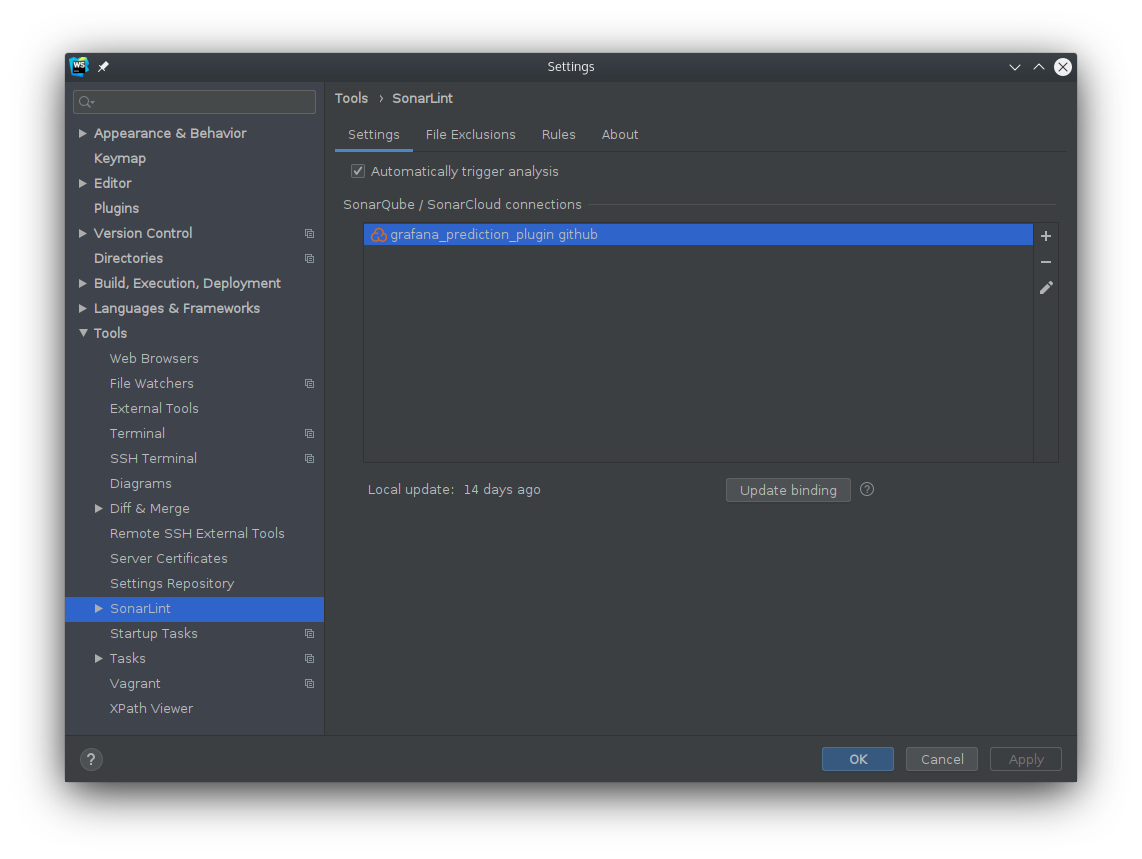
\includegraphics[width=\textwidth,height=\textheight,keepaspectratio]{img/connection.png}
Dare un nome al collegamento e selezionare SonarCloud, successivamente premere "Next".
\\
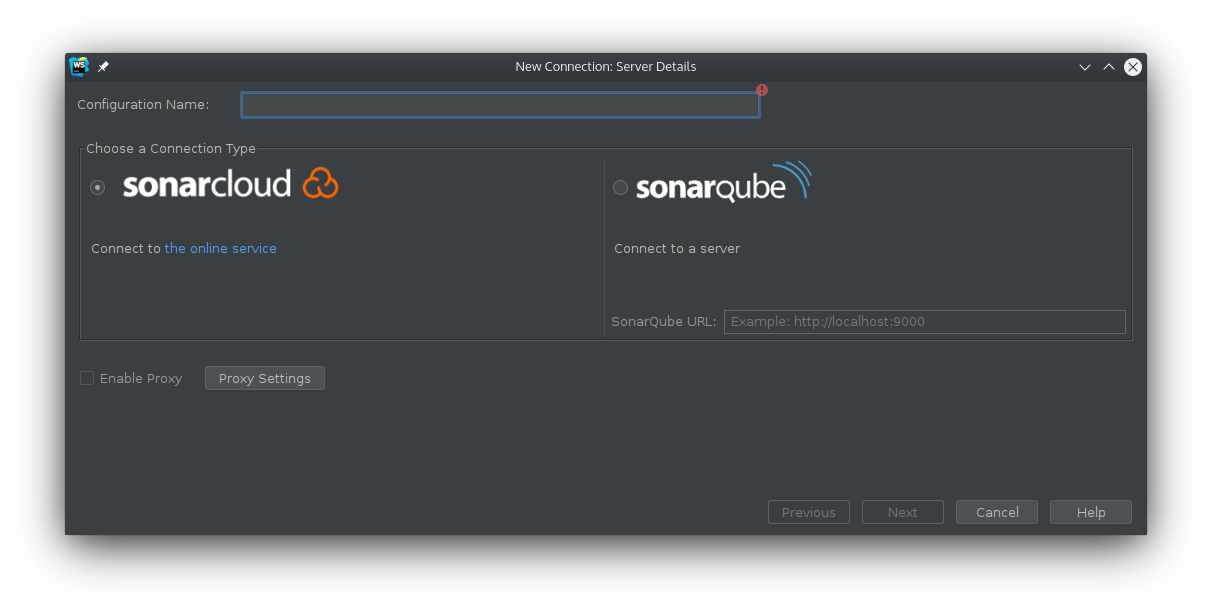
\includegraphics[width=\textwidth,height=\textheight,keepaspectratio]{img/connection-name.png}
Premere su "Create Token".
\\
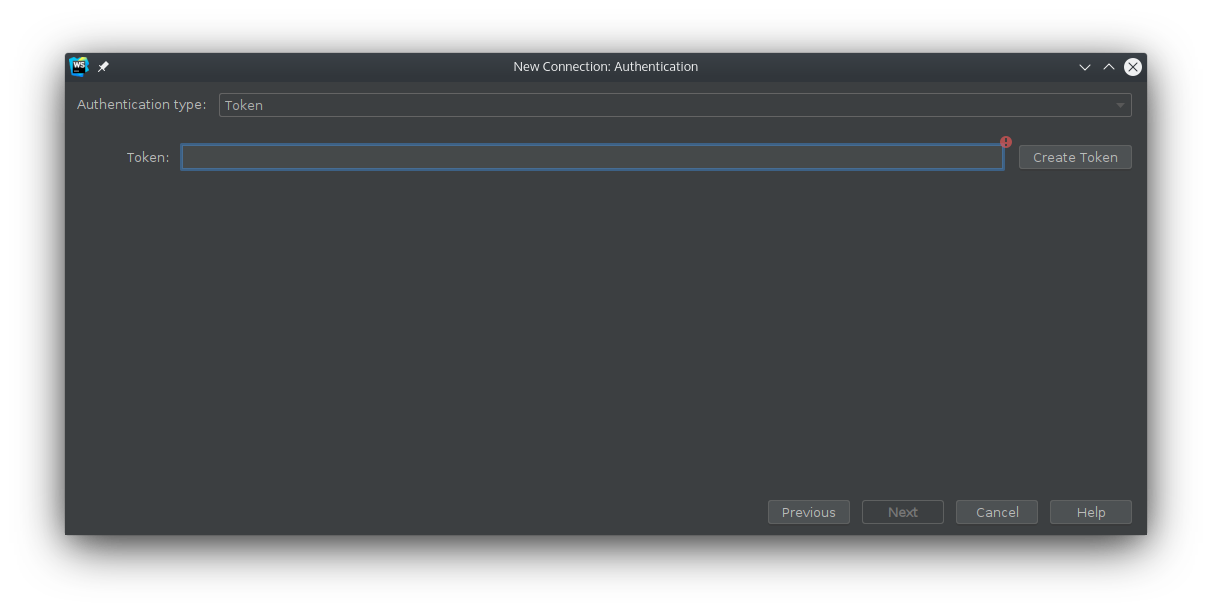
\includegraphics[width=\textwidth,height=\textheight,keepaspectratio]{img/token.png}
Scegliere un nome e creare il token, copiarlo quindi nella finestra WebStorm precedente.
\\
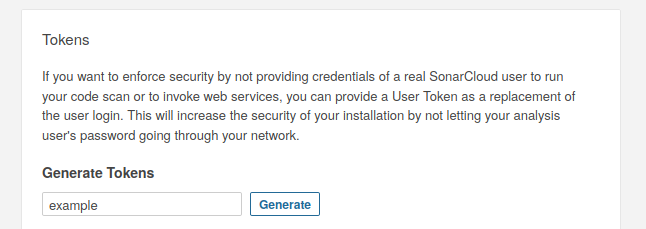
\includegraphics[width=\textwidth,height=\textheight,keepaspectratio]{img/sonarcloud.png}
La connessione verrà verificata e sarà possibile visualizzarla nell'elenco delle connessioni.
\subsubsection{Configurazione per progetto}
Dopo aver terminato la configurazione globale è possibile configurare i singoli progetti, per farlo aprire le impostazioni di WebStorm dal suo menù "File", Quindi nella sezione "Tools" espandere la voce "SonarLint" e selezionare "Project Settings".
\\
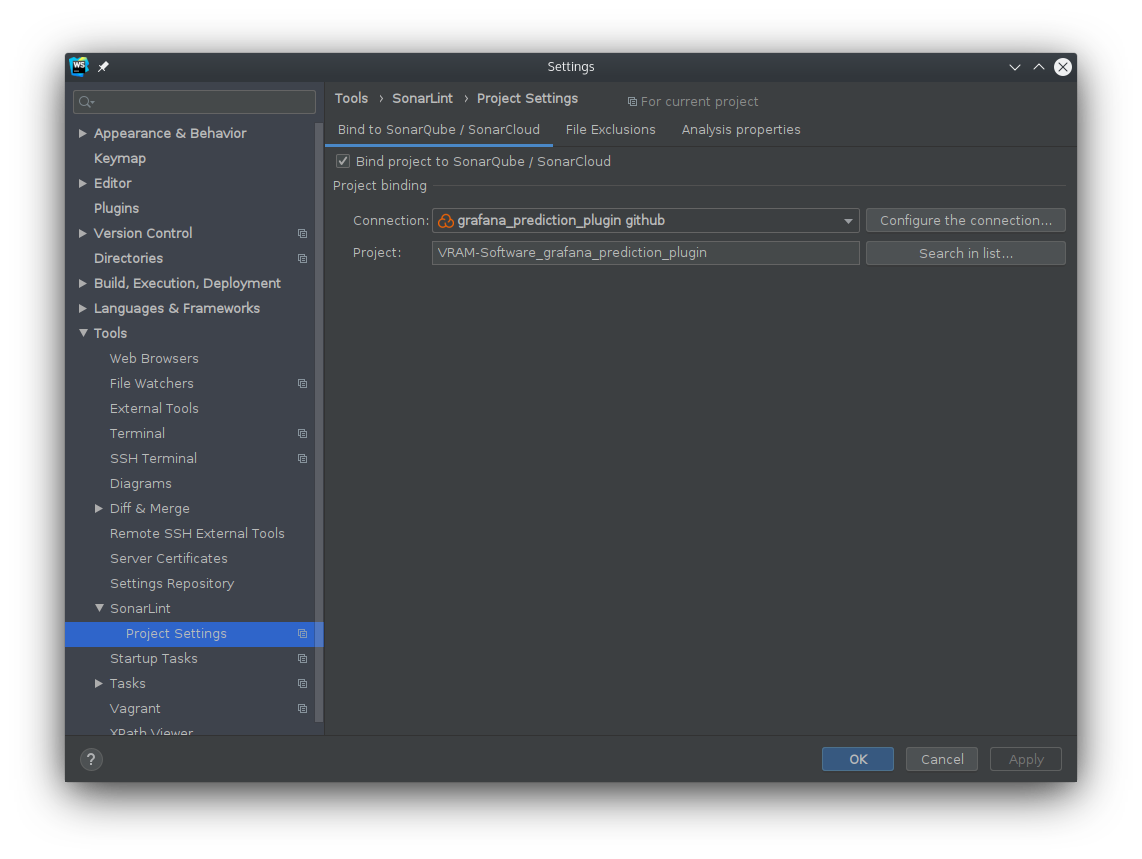
\includegraphics[width=\textwidth,height=\textheight,keepaspectratio]{img/sonarlint-project.png}
Selezionare la connessione a SonarCloud desiderata ed inserire una delle chiavi seguenti, a seconda del progetto che si sta configurando:
\begin{itemize}
	\item \textbf{plugin Grafana}: VRAM-Software\_grafana\_prediction\_plugin;
	\item \textbf{Applicativo esterno}: VRAM-Software\_prediction\_configuration\_utility.
\end{itemize}

\subsection{Configurazione ambiente plugin Grafana}
\paragraph{Contenuto file: package.json}
Il file package.json contiene tutte le informazioni e i requisiti necessari della nostra applicazione. Le informazioni importanti sono i seguenti attributi:
\textbf{"dependencies"} \\
Questo attributo contiene la seguente lista di pacchetti che sono necessari per il corretto funzionamento dell'applicazione.
\begin{itemize}
	\item jquery;
	\item lodash;
	\item moment;
	\item plotly.js;
	\item scriptjs.
\end{itemize}
\textbf{"devDependencies"} \\
Questo attributo contiene la seguente lista di pacchetti che sono necessari per il corretto funzionamento dell'applicazione durante lo sviluppo.
\begin{itemize}
	\item @grafana/data;
	\item @grafana/toolkit;
	\item @grafana/ui;
	\item @types/grafana;
	\item grafana-sdk-mocks;
	\item coveralls.
\end{itemize}
\textbf{"scripts"} \\
Questo attributo contiene una lista di tutti i comandi, utili per uno sviluppatore, che possono essere eseguiti da linea di comando.
\begin{itemize}
	\item \textbf{build}: npm run build, questo comando genera una cartella: dist che contiene i file di produzione del plugin Grafana\glo;
	\item \textbf{test}: npm test, questo comando fa eseguire tutti i test automatici dell'applicazione;
	\item \textbf{dev}: npm run dev, questo comando genera una release di debug da utilizzare durante lo sviluppo, eseguendo inoltre i linting integrati nella dipendenza npm @grafana/toolkit. Non esegue i test automatici;
	\item \textbf{ci-test}: npm run ci-test, questo comando, pensato per essere eseguito nell'ambiente di continuos integration, fa eseguire tutti i test automatici dell'applicazione e calcola il code coverage del codice;
	\item \textbf{watch}: npm run watch, questo comando esegue il comando "dev" in modalità "watch", ovvero segnalando in automatico gli errori di linting durante la scrittura del codice.
\end{itemize}
